\section{Latent Discourse Relation in Extractive Text Summarization} \label{sec:3-1}


\begin{figure}[t]
\centering
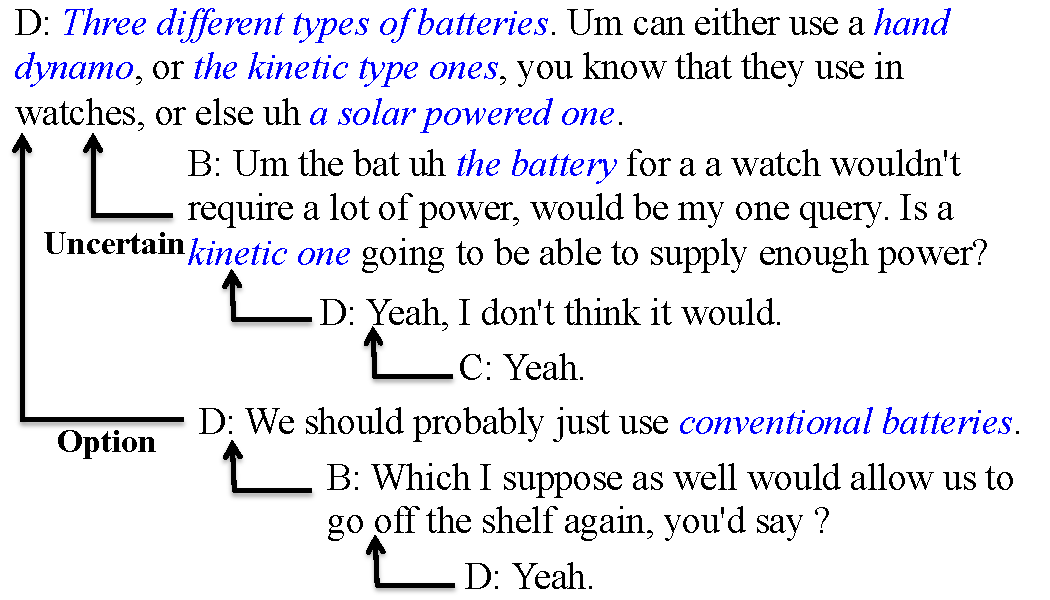
\includegraphics[width=98mm,height=60mm]{Images/snippet_intro.pdf}
%\vspace{-5mm}
\caption{ A sample clip from AMI meeting corpus. B, C, and D denotes different speakers. Here we highlight salient phrases (in \textit{italics}) that are relevant to the major topic discussed, i.e., ``which type of battery to use for the remote control''. Arrows indicate discourse structure between speaker turns. We also show some of the discourse relations for illustration.}
\label{fig:example_intro}
\end{figure}

\subsection{Background}

Goal-oriented dialogues, such as meetings, negotiations, or customer service transcripts, play an important role in our daily life. Automatically extracting the critical points and important outcomes from dialogues would facilitate generating summaries for complicated conversations, understanding the decision-making process of meetings, or analyzing the effectiveness of collaborations. In this work, we are interested in a specific type of dialogues --- spoken meetings, which is a common way for collaboration and idea sharing. Previous work~\cite{kirschner2012visualizing} has shown that discourse structure can be used to capture the main discussion points and arguments put forward during problem-solving and decision-making processes in meetings. Indeed, content of different speaker turns do not occur in isolation, and should be interpreted within the context of discourse. Meanwhile, content can also reflect the purpose of speaker turns, thus facilitate with discourse relation understanding. Take the meeting snippet from AMI corpus~\cite{ami} in Figure~\ref{fig:example_intro} as an example. This discussion is annotated with discourse structure based on the Twente Argumentation Schema (TAS) by Rutger~\cite{so65562}, which focuses on argumentative discourse information. As can be seen, meeting participants evaluate different options by showing doubt (\textsc{uncertain}), bringing up alternative solution (\textsc{option}), or giving feedback. The discourse information helps with the identification of the key discussion point, i.e., ``which type of battery to use'', by revealing the discussion flow.




% add some explanation for argumentative discourse
To date, most efforts to leverage discourse information to detect salient content from dialogues have focused on encoding gold-standard discourse relations as features for use in classifier training~\cite{murray2006incorporating,Galley:2006:SCR:1610075.1610126,mckeown2007using,Bui:2009:EDM:1708376.1708410}. However, automatic discourse parsing in dialogues is still a challenging problem~\cite{perret-EtAl:2016:N16-1}. Moreover, acquiring human annotation on discourse relations is a time-consuming and expensive process, and does not scale for large datasets. To avoid using labeled discourse features, it is natural to model discourse relation as latent variable, and use a joint modeling approach to select salient phrases reflecting key discussion points as well as label the discourse relations between speaker turns in spoken meetings. Specifically, we utilize argumentative discourse relations as defined in Twente Argument Schema (TAS)~\cite{so65562}, where discussions are organized into tree structures with discourse relations labeled between nodes (as shown in Figure~\ref{fig:example_intro}). Algorithms for joint learning and joint inference are proposed for our model. We also present a variation of our model to treat discourse relations as latent variables when true labels are not available for learning. We envision that the extracted salient phrases by our model can be used as input to abstractive meeting summarization systems~\cite{wang-cardie:2013:ACL2013,mehdad-carenini-ng:2014:P14-1}. Combined with the predicted discourse structure, a visualization tool can be exploited to display conversation flow to support intelligent meeting assistant systems.


\subsection{Jointly Modeling Content and Discourse Relations}

Our proposed model learns to jointly perform phrase-based content selection and discourse relation prediction by making use of the interaction between the two sources of information. 
%
Assume that a meeting discussion is denoted as $\mathbf{x}$, where $\mathbf{x}$ consists of a sequence of discourse units $\mathbf{x}=\{x_{1}, x_{2}, \cdots ,x_{n}\}$. Each discourse unit can be a complete speaker turn or a part of it. As demonstrated in Figure~\ref{fig:example_intro}, a tree-structured discourse diagram is constructed for each discussion with each discourse unit $x_{i}$ as a node of the tree. In this work, we consider the argumentative discourse structure by Twente Argument Schema (TAS)~\cite{so65562}. 
%
For each node $x_{i}$, it is attached to another node $x_{i^\prime}$ ($i^\prime<i$) in the discussion, and a discourse relation $d_{i}$ is hold on the link $\langle x_{i}, x_{i^\prime} \rangle$ ($d_{i}$ is empty if $x_{i}$ is the root). Let $\mathbf{t}$ denote the set of links $\langle x_{i}, x_{i^\prime} \rangle$ in $\mathbf{x}$.
%
Following previous work on discourse analysis in meetings~\cite{so65562,hakkani2009towards}, we assume that the attachment structure between discourse units are given during both training and testing. 


A set of candidate phrases are extracted from each discourse unit $x_{i}$, from which salient phrases that contain gist information will be identified. We obtain constituent and dependency parses for utterances using Stanford parser~\cite{Klein:2003:AUP:1075096.1075150}. We restrict eligible candidate to be a noun phrase (NP), verb phrase (VP), prepositional phrase (PP), or adjective phrase (ADJP) with at most 5 words, and its head word cannot be a stop word.\footnote{Other methods for mining candidate phrases, such as frequency-based method~\cite{liu2015mining}, will be studied for future work.} 
If a candidate is a parent of another candidate in the constituent parse tree, we will only keep the parent. We further merge a verb and a candidate noun phrase into one candidate if the later is the direct object or subject of the verb. For example, from utterance ``let's use a rubber case as well as rubber buttons'', we can identify candidates ``use a rubber case'' and ``rubber buttons''. 
For $x_{i}$, the set of candidate phrases are denoted as $c_{i}=\{c_{i,1},c_{i,2},\cdots,c_{i,m_i}\}$, where $m_i$ is the number of candidates. $c_{i,j}$ takes a value of $1$ if the corresponding candidate is selected as salient phrase; otherwise, $c_{i,j}$ is equal to $0$. All candidate phrases in discussion $\mathbf{x}$ are represented as $\mathbf{c}$.

%In this work, we focus on identifying salient phrases which contain gist information during a meeting, and predicting the discourse relations hold between discourse units. 

We then define a log-linear model with feature parameters $\mathbf{w}$ for the candidate phrases $\mathbf{c}$ and discourse relations $\mathbf{d}$ in $\mathbf{x}$ as:

%\vspace{-5mm}
{\fontsize{10}{10}\selectfont
\begin{equation}
\begin{split}
& p(\mathbf{c}, \mathbf{d}|\mathbf{x}, \mathbf{w}) \propto \exp [\mathbf{w}\cdot \Phi (\mathbf{c}, \mathbf{d}, \mathbf{x})] \propto \exp [\mathbf{w}\cdot \sum_{i=1, <x_i, x_{i^\prime}>\in \mathbf{t}}^{n} \phi (c_{i}, d_{i}, d_{i^\prime}, \mathbf{x})]\\
& \propto \exp [\sum_{i=1,<x_i, x_{i^\prime}>\in \mathbf{t}}^{n} ( \mathbf{w_c}\cdot \sum_{j=1}^{m_i} \phi_c (c_{i,j}, \mathbf{x})+ \mathbf{w_d}\cdot \phi_d (d_{i},d_{i^\prime}, \mathbf{x}) + \mathbf{w_{cd}}\cdot \sum_{j=1}^{m_i} \phi_{cd} (c_{i,j}, d_{i}, \mathbf{x}) ) ]\\
\end{split}
\end{equation}
\label{eq:objective}
}
%
Here $\Phi(\cdot)$ and $\phi(\cdot)$ denote feature vectors. We utilize three types of feature functions: (1) content-only features $\phi_c(\cdot)$, which capture the importance of phrases, (2) discourse-only features $\phi_d(\cdot)$, which characterize the (potentially higher-order) discourse relations, and (3) joint features of content and discourse $\phi_{cd}(\cdot)$, which model the interaction between the two. $\mathbf{w_c}$, $\mathbf{w_d}$, and $\mathbf{w_{cd}}$ are corresponding feature parameters. Detailed feature descriptions can be found in appendix \ref{sec:feature}. 

Acquiring labeled training data for discourse relations is a time-consuming process since it would require human annotators to inspect the full discussions. Therefore, we further propose a variation of our model where it treats the discourse relations as latent variables, so that $p(\mathbf{c} |\mathbf{x}, \mathbf{w})=\sum_{\mathbf{d}} p(\mathbf{c}, \mathbf{d}|\mathbf{x}, \mathbf{w})$. Its learning algorithm is slightly different as described latter. For learning the model parameters $\mathbf{w}$, we employ an algorithm based on SampleRank~\cite{rohanimanesh2011samplerank}, which is a stochastic structure learning method. In general, the learning algorithm constructs a sequence of configurations for sample labels as a Markov chain Monte Carlo (MCMC) chain based on a task-specific loss function, where stochastic gradients are distributed across the chain. %This is suitable for our learning problem because we aim to optimize the prediction performance for both phrase selection and discourse relations with various types of features.

The full learning procedure is described in Algorithm~\ref{alg:learning}. To start with, the feature weights $\mathbf{w}$ is initialized with each value randomly drawn from $[-1, 1]$. Multiple epochs are run through all samples. 
For each sample, we randomly initialize the assignment of candidate phrases labels $\mathbf{c}$ and discourse relations $\mathbf{d}$. 
%
Then an MCMC chain is constructed with a series of configurations $\sigma =(\mathbf{c}$, $\mathbf{d})$: at each step, it first samples a discourse structure $\mathbf{d}$ based on the proposal distribution $q(\mathbf{d^\prime} |\mathbf{d},\mathbf{x})$, and then samples phrase labels conditional on the new discourse relations and previous phrase labels based on $q(\mathbf{c^\prime} |\mathbf{c}, \mathbf{d^\prime},\mathbf{x})$. Local search is used for both proposal distributions.\footnote{For future work, we can explore other proposal distributions that utilize the conditional distribution of salient phrases given sampled discourse relations.}   
%
The new configuration is accepted if it improves on the score by $\omega (\sigma ^\prime)$. The parameters $\mathbf{w}$ are updated accordingly. For the scorer $\omega$, we use a weighted combination of F1 scores of phrase selection ($F1_{c}$) and discourse relation prediction ($F1_{d}$): $\omega (\sigma)= \alpha \cdot F1_{c} +  (1-\alpha) \cdot F1_{d}$. We fix $\alpha$ to $0.1$. When discourse relations are treated as latent, we initialize discourse relations for each sample with a label in $\{1, 2, \ldots, K\}$ if there are $K$ relations indicated, and we only use $F1_{c}$ as the scorer.
%We only use F1 score of phrase selection as our scorer.


\begin{algorithm}[t]
{
\SetKwInOut{Input}{Input}
\SetKwInOut{Output}{Output}

\Input{$\mathbf{X}=\{\mathbf{x}\}$: discussions in the training set, \\
	$\eta$: learning rate, 
	$\epsilon$: number of epochs, \\
	$\delta$: number of sampling rounds, \\
	$\omega (\cdot)$: scoring function,
	$\Phi (\cdot)$: feature functions
	}

\Output{feature weights $\frac{1}{|\mathcal{W}|}\sum_{\mathbf{w}\in \mathcal{W}} \mathbf{w}$}
\BlankLine

Initialize $\mathbf{w}$\;
$\mathcal{W} \leftarrow \{\mathbf{w} \}$\;

\For {$e=1$ to $\epsilon$} {

	\For {$\mathbf{x}$ in $\mathbf{X}$} {
	
		\tcp{Initialize configuration for $\mathbf{x}$}
		Initialize $\mathbf{c}$ and $\mathbf{d}$\;
		$\sigma=(\mathbf{c}, \mathbf{d})$\;
		\For {$s=1$ to $\delta$} {
			\tcp{New configuration via local search}
			$\mathbf{d^\prime} \sim q_d(\cdot | \mathbf{x}, \mathbf{d})$\;
			$\mathbf{c^\prime} \sim q_d(\cdot | \mathbf{x}, \mathbf{c}, \mathbf{d^\prime})$\;
			
			$\sigma^\prime=(\mathbf{c^\prime}, \mathbf{d^\prime})$\;
			
			$\sigma^+=\arg \max_{\tilde{\sigma} \in \{\sigma, \sigma^\prime \}} \omega (\tilde{\sigma}) $\;
			$\sigma^-=\arg \min_{\tilde{\sigma} \in \{\sigma, \sigma^\prime \}} \omega (\tilde{\sigma}) $\;		
			
			$\hat{\nabla}=\Phi (\sigma^+)- \Phi (\sigma^-)$\;
			$\Delta \omega= \omega (\sigma^+)- \omega (\sigma^-)$\; 

			\tcp{Update parameters}			
			\If {$\mathbf{w}\cdot \hat{\nabla} < \Delta \omega$ \& $\Delta \omega\neq 0$}{
				$\mathbf{w} \leftarrow \mathbf{w}+\eta \cdot \hat{\nabla}$\;
				Add $\mathbf{w}$ in $\mathcal{W}$\;
			}
			
			\tcp{Accept or reject new configuration}
			\If {$\sigma^+ == \sigma^\prime$}{
				$\sigma=\sigma^\prime$
			
			}
		}
	
	}
}
}

\caption{\fontsize{10}{12}\selectfont  SampleRank-based joint learning.}
\label{alg:learning}
\end{algorithm}

Given a new sample $\mathbf{x}$ and learned parameters $\mathbf{w}$, we predict phrase labels and discourse relations as $\arg \max_{\mathbf{c}, \mathbf{d}} p(\mathbf{c}, \mathbf{d}|\mathbf{x}, \mathbf{w})$. Dynamic programming can be employed to carry out joint inference, however, it would be time-consuming since our objective function has a large search space for both content and discourse labels. Hence we propose an alternating optimizing algorithm to search for $\mathbf{c}$ and $\mathbf{d}$ iteratively. Concretely, for each iteration, we first optimize on $\mathbf{d}$ by maximizing $\sum_{i=1,<x_i, x_i^\prime>\in \mathbf{t}}^{n} (\mathbf{w_d}\cdot \phi_d (d_{i},d_{i^\prime}, \mathbf{x}) + \mathbf{w_{cd}}\cdot \sum_{j=1}^{m_i} \phi_{cd} (c_{i,j}, d_{i}, \mathbf{x}))$. Message-passing~\cite{smith2008dependency} is used to find the best $\mathbf{d}$.

In the second step, we search for $\mathbf{c}$ that maximizes $\sum_{i=1,<x_i, x_i^\prime>\in \mathbf{t}}^{n} (\mathbf{w_c}\cdot \sum_{j=1}^{m_i} \phi_c (c_{i,j}, \mathbf{x}) + \mathbf{w_{cd}}\cdot \sum_{j=1}^{m_i} \phi_{cd} (c_{i,j}, d_{i}, \mathbf{x}) )$. We believe that candidate phrases based on the same concepts should have the same predicted label. Therefore, candidates of the same phrase type and sharing the same head word are grouped into one cluster. We then cast our task as an integer linear programming problem.\footnote{We use lpsolve: \url{http://lpsolve.sourceforge.net/5.5/}.} We optimize our objective function under constraints: (1) $c_{i,j}=c_{i^\prime, j^\prime}$ if $c_{i,j}$ and $c_{i^\prime, j^\prime}$ are in the same cluster, and (2) $c_{i,j}\in \{0, 1\} $, $\forall i, j$. The inference process is the same for models trained with latent discourse relations.

We evaluate our joint model on the AMI meeting corpus~\cite{ami}, where consists of 139 scenario-driven meetings and labeled with gold-standard discourse relations and summaries. Two variations of our joint model are tested: one is trained on gold-standard discourse relations, the other is trained by treating discourse relations as latent variables, and these two  methods are henceforth referred as \textit{Our Model} and \textit{Our Model-latent}. 

We evaluate whether the prediction of the content selection component can be used for summarizing the key points on discussion level. For each discussion, salient phrases identified by our model are concatenated in sequence for use as the summary. We consider two types of gold-standard summaries. One is utterance-level extractive summary, which consists of human labeled summary-worthy utterances. The other is abstractive summary, where we collect human abstract with at least one link from summary-worthy utterances.

\begin{table}[ht]

\parbox{.47\linewidth}{\fontsize{8}{9}\selectfont
\setlength{\tabcolsep}{0.8mm}
\begin{tabular}{|l|l|l|l|l|l|l|l|}

\hline

	\multicolumn{8}{|l|}{\textit{Extractive Summaries as Gold-Standard}}\\ \hline
    & &\multicolumn{3}{c|}{\textsc{ROUGE-1}} & \multicolumn{3}{c|}{\textsc{ROUGE-SU4}}\\ \hline
    & Len & Prec & Rec & F1 & Prec & Rec & F1\\ 
%   \underline{\textbf{Comparisons}} & & & & & & &  \\ 
	Longest DA & 30.9 & 64.4 & 15.0  & 23.1 & 58.6 & 9.3 & 15.3 \\ 
   	Centroid DA & 17.5 & {\bf 73.9} & 13.4 & 20.8 & {\bf 62.5} & 6.9 & 11.3 \\ 
	SVM & 49.8& 47.1 & 24.1 & 27.5 & 22.7 & 10.7 & 11.8 \\ 
    Liu \cite{liu2009unsupervised} & 62.4& 40.4 & 39.2 & 36.2 & 15.5 & 15.2 & 13.5 \\ 
    \hline\hline
	Our Model & 66.6 & 45.4 & 44.7 & 41.1$\ast$ & 24.1$\ast$ & 23.4$\ast$ & 20.9$\ast$ \\ 
   	Our Model-latent & 85.9 & 42.9 & {\bf 49.3} & {\bf 42.4}$\ast$ & 21.6 & {\bf 25.7}$\ast$ & {\bf 21.3}$\ast$ \\ 
   
 \hline\hline

	\multicolumn{8}{|l|}{\textit{Abstractive Summaries as Gold-Standard}}\\ \hline
    & &\multicolumn{3}{c|}{\textsc{ROUGE1}} & \multicolumn{3}{c|}{\textsc{ROUGE-SU4}}\\ \hline
    &  Len & Prec & Rec & F1 & Prec & Rec & F1\\ 
%   \underline{\textbf{Comparisons}} & & & & & & &  \\ 
	Longest DA & 30.9 & 14.8  & 5.5 & 7.4 & 4.8 & 1.4 & 1.9 \\ 
   	Centroid DA & 17.5 &{\bf 24.9} &  5.6 & 8.5 & {\bf 11.6} & 1.4 & 2.2 \\ 
   	SVM & 49.8& 13.3& 9.7  & 9.5 & 4.4 & 2.4 & 2.4 \\ 
    Liu \cite{liu2009unsupervised} & 62.4& 10.3 & 16.7 & 11.3 & 2.7 & 4.5 & 2.8 \\ 
    \hline\hline
    
	Our Model & 66.6& 12.6 & 18.9 & {\bf 13.1}$\ast$ & 3.8 & 5.5$\ast$ & {\bf 3.7}$\ast$ \\ 
	Our Model-latent & 85.9 & 11.4 & {\bf 20.0} & 12.4$\ast$ & 3.3 & {\bf 6.1}$\ast$ & 3.5$\ast$ \\ 
   
    \hline
\end{tabular}
\caption{\fontsize{10}{12}\selectfont ROUGE scores for phrase-based extractive summarization evaluated against human-constructed utterance-level extractive summaries and abstractive summaries. Our models that statistically significantly outperform SVM and Liu \cite{liu2009unsupervised} are highlighted with $\ast$ ($p < 0.05$, paired $t$-test). Best ROUGE score for each column is in \textbf{bold}.}
\label{tab:summ}
}
\hfill
\parbox{.50\linewidth}{
\centering
	{\fontsize{8}{9}\selectfont
    \setlength{\tabcolsep}{0.6mm}
%    \hspace{-2mm}
    \begin{tabular}{|p{75mm}|}
    \hline
	
	\textbf{Meeting Clip}: \\
	D: can we uh power a light in this? can we get a strong enough battery to power a light? \\
	A: um i think we could because the lcd panel requires power, and the lcd is a form of a light so that$\ldots$\\
	D: $\ldots$it's gonna have to have something high-tech about it and that's gonna take battery power$\ldots$ \\
	D: illuminate the buttons. yeah it glows.\\
	D: well m i'm thinking along the lines of you're you're in the dark watching a dvd and you um you find the thing in the dark and you go like this $\ldots$ oh where's the volume button in the dark, and uh y you just touch it $\ldots$ and it lights up or something.\\

	\hline \hline    
    
	\textbf{Abstract by Human}: \\
    What sort of battery to use. The industrial designer presented options for materials, components, and batteries and discussed the restrictions involved in using certain materials.\\
	
	\hline \hline
	
	\textbf{Longest DA}: \\
	well m i'm thinking along the lines of you're you're in the dark watching a dvd and you um you find the thing in the dark and you go like this.\\
	\textbf{Centroid DA}: \\
	can we uh power a light in this?\\

	\textbf{Our Method}: \\
	- power a light, a strong enough battery, \\
	- requires power, a form, \\
	- a really good battery, battery power, \\
	- illuminate the buttons, glows, \\
	- watching a dvd, the volume button, lights up or something\\	
    \hline
    \end{tabular}
    
    }
	\caption{\fontsize{10}{12}\selectfont Sample summaries output by different systems for a meeting clip from AMI corpus (less relevant utterances in between are removed). Salient phrases by our system output are displayed for each turn of the clip, with duplicated phrases removed for brevity. }%Our system summary captures argumentation process and important outcomes of the discussion.}
\label{fig:example_summary}
}
\end{table}




% metrics
We calculate scores based on ROUGE~\cite{Lin:2003:AES:1073445.1073465}, which is a popular tool for evaluating text summarization~\cite{gillick2009global,liu2010using}. ROUGE-1 (unigrams) and ROUGE-SU4 (skip-bigrams with at most 4 words in between) are used. 
%The ROUGE scores are computed by using official ROUOGE software with standard options.\footnote{ROUGE option: -n 4 -w 1.2 -m -2 4 -u -c 95 -r 1000 -f A -p 0.5 -t 0 -a -d} 
% baselines and comparison
Following previous work on meeting summarization~\cite{Riedhammer:2010:LSS:1837521.1837625,wang-cardie:2013:ACL2013}, we consider two dialogue act-level summarization baselines: (1) \textsc{longest DA} in each discussion is selected as the summary, and (2) \textsc{centroid DA}, the one with the highest TF-IDF similarity with all DAs in the discussion. 
%
We also compare with an unsupervised keyword extraction approach by Liu \cite{liu2009unsupervised}, where word importance is estimated by its TF-IDF score, POS tag, and the salience of its corresponding sentence. With the same candidate phrases as in our model, we extend Liu \cite{liu2009unsupervised} by scoring each phrase based on its average score of the words. Top phrases, with the same number of phrases output by our model, are included into the summaries. 
%
Finally, we compare with summaries consisting of salient phrases predicted by an SVM classifier trained with our content features.

From the results in Table~\ref{tab:summ}, we can see that phrase-based extractive summarization methods can yield better ROUGE scores for recall and F1 than baselines that extract the whole sentences. 
%
Meanwhile, our system significantly outperforms the SVM-based classifiers when evaluated on ROUGE recall and F1, while achieving comparable precision. Compared to Liu \cite{liu2009unsupervised}, our system also yields better results on all metrics.

Sample summaries by our model along with two baselines are displayed in Table~\ref{fig:example_summary}. Utterance-level extract-based baselines unavoidably contain disfluency and unnecessary details. Our phrase-based extractive summary is able to capture the key points from both the argumentation process and important outcomes of the conversation. This implies that our model output can be used as input for an abstractive summarization system. It can also facilitate the visualization of decision-making processes.



\subsection{Predicting Consistency of Understanding}
As discussed in previous work~\cite{mulder2002assessing,mercer2004sociocultural}, both content and discourse structure are critical for building shared understanding among discussants. 
In this section, we test whether our joint model can be utilized to predict the consistency among team members' understanding of their group decisions, which is defined as consistency of understanding (COU) in Kim \cite{kim2016improving}. This downstream task can also be used to evaluate the correctness of the generated discourse structures.%with an objective to develop intelligent systems that can suggest review of topics potentially resulting in inconsistent understandings among participants.

Kim \cite{kim2016improving} establish gold-standard COU labels on a portion of AMI discussions, by comparing participant summaries to determine whether participants report the same decisions. If all decision points are consistent, the associated topic discussion is labeled as \textit{consistent}; otherwise, the discussion is identified as \textit{inconsistent}. Their annotation covers a subset transcripts in the \textsc{AMI} dataset (we shall call it \textsc{AMI-sub}). Therefore, we run the prediction experiments on \textsc{AMI-sub} by using the same annotation. 
Out of total 129 discussions in \textsc{AMI-sub}, 86 discussions are labeled as consistent and 43 are inconsistent. 

We construct three types of features by using our model's predicted labels. Firstly, we learn two versions of our model based on the ``consistent'' discussions and the ``inconsistent'' ones in the training set, with learned parameters $\mathbf{w_{con}}$ and $\mathbf{w_{incon}}$. For a discussion in the test set, these two models output two probabilities $p_{con}=\max_{\mathbf{c}, \mathbf{d}} P(\mathbf{c}, \mathbf{d}|\mathbf{x}, \mathbf{w_{con}})$ and $p_{incon}=\max_{\mathbf{c}, \mathbf{d}} P(\mathbf{c}, \mathbf{d}|\mathbf{x}, \mathbf{w_{incon}})$. We use $p_{con}-p_{incon}$ as a feature. Furthermore, we consider discourse relations of length one and two from the discourse structure tree. Intuitively, some discourse relations, e.g., \textsc{elaboration} followed by multiple \textsc{positive} feedback, imply consistent understanding. The third feature is based on word entrainment, which has been shown to correlate with task success for groups~\cite{nenkova2008high}. Using the formula in Nenkova~\cite{nenkova2008high}, we compute the average word entrainment between the main speaker who utters the most words and all the other participants. The content words in the salient phrases predicted by our model is considered for entrainment computation.


\begin{table}[t]
\centering
\fontsize{9}{10}\selectfont
%\setlength{\baselineskip}{0pt}
\setlength{\tabcolsep}{1.5mm}
\begin{tabular}{|l|c|c|}
    \hline
%         &\multicolumn{2}{c|}{\textbf{SVM}}\\ 
        & \textbf{Acc} & \textbf{F1} \\ \hline
        \underline{\textbf{Comparisons}} && \\
        Baseline (Majority) & 66.7 & 40.0  \\ 
%        Baseline (Random) & 50.0 & 32.3\\ 
        Ngrams (SVM) & 51.2 & 50.6  \\ 
        %Kim \& Shah & 60.5 & 50.5 \\ \hline\hline
		Kim \cite{kim2016improving} & 60.5 & 50.5 \\ \hline\hline
		        
        \underline{\textbf{Features from Our Model}}&&  \\ 
        Consistency Probability (Prob) & 52.7 & 52.1 \\ 
        Discourse Relation (Disc) & 63.6 & 57.1$\ast$  \\ 
        Word Entrainment (Ent) & 60.5$\ast$ & 57.1$\ast$\\ 
        Prob + Disc+ Ent & {\bf 68.2}$\ast$ & {\bf 63.1}$\ast$  \\ \hline\hline

        \underline{\textbf{Oracles}}&&  \\ 
        Discourse Relation & 69.8 & 62.7 \\ 
        Word Entrainment & 61.2 & 57.8 \\ \hline
\end{tabular}
\caption{Consistency of Understanding (COU) prediction results on \textsc{AMI-sub}. Results that statistically significantly outperform ngrams-based baseline and Kim \cite{kim2016improving} are highlighted with $\ast$ ($p < 0.05$, paired $t$-test). %Best result (excluding oracles) for each column is in \textbf{bold}. 
For reference, we also show the prediction performance based on gold-standard discourse relations and phrase selection labels.}
\label{tab:consistency}
\end{table}

\noindent \textbf{Results.} 
Leave-one-out is used for experiments. For training, our features are constructed from gold-standard phrase and discourse labels. Predicted labels by our model is used for constructing features during testing. SVM-based classifier is used for experimenting with different sets of features output by our model. 
A majority class baseline is constructed as well. We also consider an SVM classifier trained with ngram features (unigrams and bigrams). Finally, we compare with the state-of-the-art method in Kim ~\cite{kim2016improving}, where discourse-relevant features and head gesture features are utilized in Hidden Markov Models to predict the consistency label.

The results are displayed in Table~\ref{tab:consistency}. All SVMs trained with our features surpass the ngrams-based baseline. Especially, the discourse features, word entrainment feature, and the combination of the three, all significantly outperform the state-of-the-art system by Kim \cite{kim2016improving}.\footnote{We also experiment with other popular classifiers, e.g. logistic regression or decision tree, and similar trend is respected.}


